\documentclass[1p]{elsarticle_modified}
%\bibliographystyle{elsarticle-num}

%\usepackage[colorlinks]{hyperref}
%\usepackage{abbrmath_seonhwa} %\Abb, \Ascr, \Acal ,\Abf, \Afrak
\usepackage{amsfonts}
\usepackage{amssymb}
\usepackage{amsmath}
\usepackage{amsthm}
\usepackage{scalefnt}
\usepackage{amsbsy}
\usepackage{kotex}
\usepackage{caption}
\usepackage{subfig}
\usepackage{color}
\usepackage{graphicx}
\usepackage{xcolor} %% white, black, red, green, blue, cyan, magenta, yellow
\usepackage{float}
\usepackage{setspace}
\usepackage{hyperref}

\usepackage{tikz}
\usetikzlibrary{arrows}

\usepackage{multirow}
\usepackage{array} % fixed length table
\usepackage{hhline}

%%%%%%%%%%%%%%%%%%%%%
\makeatletter
\renewcommand*\env@matrix[1][\arraystretch]{%
	\edef\arraystretch{#1}%
	\hskip -\arraycolsep
	\let\@ifnextchar\new@ifnextchar
	\array{*\c@MaxMatrixCols c}}
\makeatother %https://tex.stackexchange.com/questions/14071/how-can-i-increase-the-line-spacing-in-a-matrix
%%%%%%%%%%%%%%%

\usepackage[normalem]{ulem}

\newcommand{\msout}[1]{\ifmmode\text{\sout{\ensuremath{#1}}}\else\sout{#1}\fi}
%SOURCE: \msout is \stkout macro in https://tex.stackexchange.com/questions/20609/strikeout-in-math-mode

\newcommand{\cancel}[1]{
	\ifmmode
	{\color{red}\msout{#1}}
	\else
	{\color{red}\sout{#1}}
	\fi
}

\newcommand{\add}[1]{
	{\color{blue}\uwave{#1}}
}

\newcommand{\replace}[2]{
	\ifmmode
	{\color{red}\msout{#1}}{\color{blue}\uwave{#2}}
	\else
	{\color{red}\sout{#1}}{\color{blue}\uwave{#2}}
	\fi
}

\newcommand{\Sol}{\mathcal{S}} %segment
\newcommand{\D}{D} %diagram
\newcommand{\A}{\mathcal{A}} %arc


%%%%%%%%%%%%%%%%%%%%%%%%%%%%%5 test

\def\sl{\operatorname{\textup{SL}}(2,\Cbb)}
\def\psl{\operatorname{\textup{PSL}}(2,\Cbb)}
\def\quan{\mkern 1mu \triangleright \mkern 1mu}

\theoremstyle{definition}
\newtheorem{thm}{Theorem}[section]
\newtheorem{prop}[thm]{Proposition}
\newtheorem{lem}[thm]{Lemma}
\newtheorem{ques}[thm]{Question}
\newtheorem{cor}[thm]{Corollary}
\newtheorem{defn}[thm]{Definition}
\newtheorem{exam}[thm]{Example}
\newtheorem{rmk}[thm]{Remark}
\newtheorem{alg}[thm]{Algorithm}

\newcommand{\I}{\sqrt{-1}}
\begin{document}

%\begin{frontmatter}
%
%\title{Boundary parabolic representations of knots up to 8 crossings}
%
%%% Group authors per affiliation:
%\author{Yunhi Cho} 
%\address{Department of Mathematics, University of Seoul, Seoul, Korea}
%\ead{yhcho@uos.ac.kr}
%
%
%\author{Seonhwa Kim} %\fnref{s_kim}}
%\address{Center for Geometry and Physics, Institute for Basic Science, Pohang, 37673, Korea}
%\ead{ryeona17@ibs.re.kr}
%
%\author{Hyuk Kim}
%\address{Department of Mathematical Sciences, Seoul National University, Seoul 08826, Korea}
%\ead{hyukkim@snu.ac.kr}
%
%\author{Seokbeom Yoon}
%\address{Department of Mathematical Sciences, Seoul National University, Seoul, 08826,  Korea}
%\ead{sbyoon15@snu.ac.kr}
%
%\begin{abstract}
%We find all boundary parabolic representation of knots up to 8 crossings.
%
%\end{abstract}
%\begin{keyword}
%    \MSC[2010] 57M25 
%\end{keyword}
%
%\end{frontmatter}

%\linenumbers
%\tableofcontents
%
\newcommand\colored[1]{\textcolor{white}{\rule[-0.35ex]{0.8em}{1.4ex}}\kern-0.8em\color{red} #1}%
%\newcommand\colored[1]{\textcolor{white}{ #1}\kern-2.17ex	\textcolor{white}{ #1}\kern-1.81ex	\textcolor{white}{ #1}\kern-2.15ex\color{red}#1	}

{\Large $\underline{12a_{1224}~(K12a_{1224})}$}

\setlength{\tabcolsep}{10pt}
\renewcommand{\arraystretch}{1.6}
\vspace{1cm}\begin{tabular}{m{100pt}>{\centering\arraybackslash}m{274pt}}
\multirow{5}{120pt}{
	\centering
	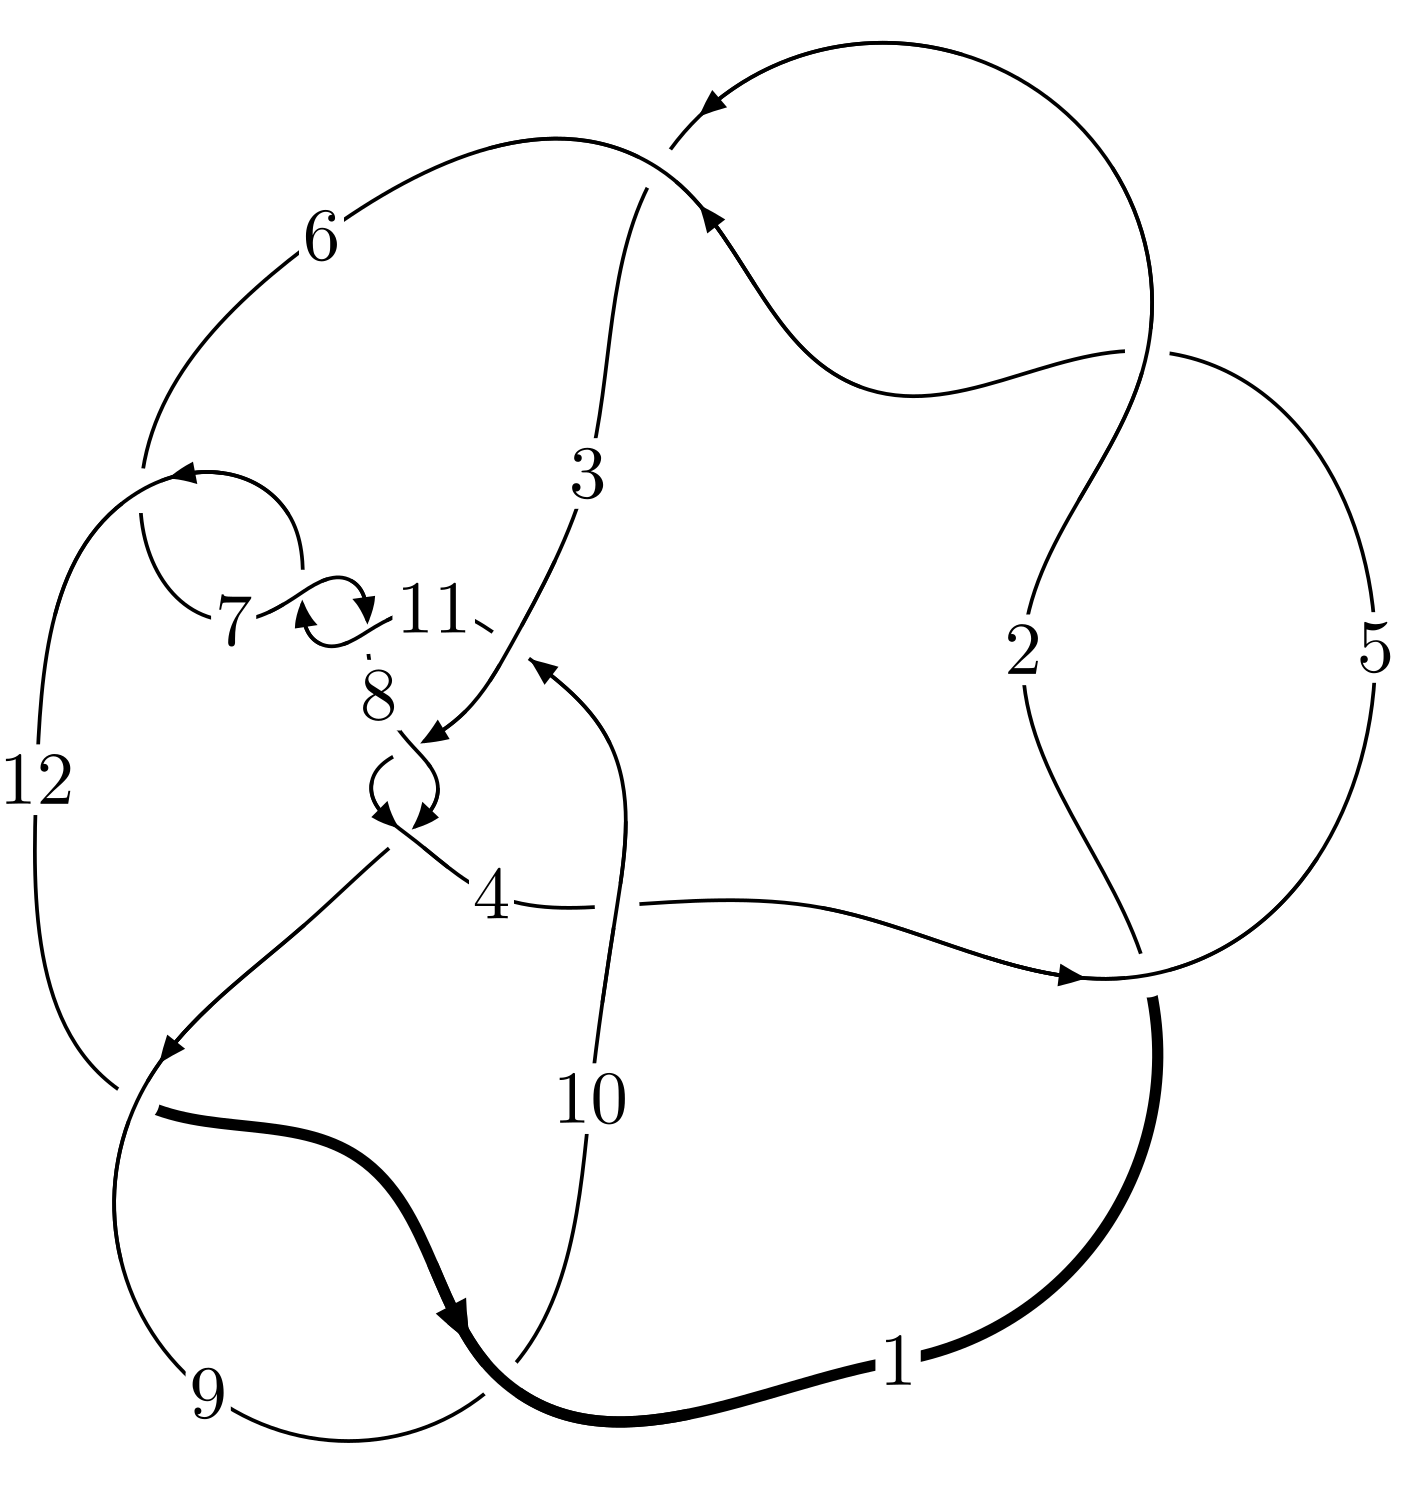
\includegraphics[width=112pt]{../../../GIT/diagram.site/Diagrams/png/2025_12a_1224.png}\\
\ \ \ A knot diagram\footnotemark}&
\allowdisplaybreaks
\textbf{Linearized knot diagam} \\
\cline{2-2}
 &
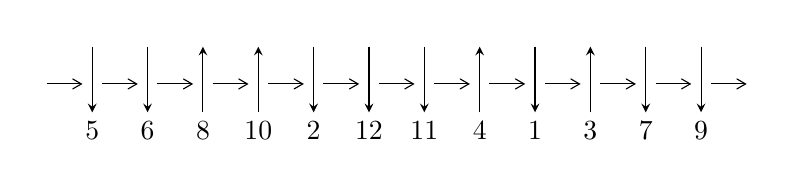
\begin{tikzpicture}[x=20pt, y=17pt]
	% nodes
	\node (C0) at (0, 0) {};
	\node (C1) at (1, 0) {};
	\node (C1U) at (1, +1) {};
	\node (C1D) at (1, -1) {5};

	\node (C2) at (2, 0) {};
	\node (C2U) at (2, +1) {};
	\node (C2D) at (2, -1) {6};

	\node (C3) at (3, 0) {};
	\node (C3U) at (3, +1) {};
	\node (C3D) at (3, -1) {8};

	\node (C4) at (4, 0) {};
	\node (C4U) at (4, +1) {};
	\node (C4D) at (4, -1) {10};

	\node (C5) at (5, 0) {};
	\node (C5U) at (5, +1) {};
	\node (C5D) at (5, -1) {2};

	\node (C6) at (6, 0) {};
	\node (C6U) at (6, +1) {};
	\node (C6D) at (6, -1) {12};

	\node (C7) at (7, 0) {};
	\node (C7U) at (7, +1) {};
	\node (C7D) at (7, -1) {11};

	\node (C8) at (8, 0) {};
	\node (C8U) at (8, +1) {};
	\node (C8D) at (8, -1) {4};

	\node (C9) at (9, 0) {};
	\node (C9U) at (9, +1) {};
	\node (C9D) at (9, -1) {1};

	\node (C10) at (10, 0) {};
	\node (C10U) at (10, +1) {};
	\node (C10D) at (10, -1) {3};

	\node (C11) at (11, 0) {};
	\node (C11U) at (11, +1) {};
	\node (C11D) at (11, -1) {7};

	\node (C12) at (12, 0) {};
	\node (C12U) at (12, +1) {};
	\node (C12D) at (12, -1) {9};
	\node (C13) at (13, 0) {};

	% arrows
	\draw[->,>={angle 60}]
	(C0) edge (C1) (C1) edge (C2) (C2) edge (C3) (C3) edge (C4) (C4) edge (C5) (C5) edge (C6) (C6) edge (C7) (C7) edge (C8) (C8) edge (C9) (C9) edge (C10) (C10) edge (C11) (C11) edge (C12) (C12) edge (C13) ;	\draw[->,>=stealth]
	(C1U) edge (C1D) (C2U) edge (C2D) (C3D) edge (C3U) (C4D) edge (C4U) (C5U) edge (C5D) (C6U) edge (C6D) (C7U) edge (C7D) (C8D) edge (C8U) (C9U) edge (C9D) (C10D) edge (C10U) (C11U) edge (C11D) (C12U) edge (C12D) ;
	\end{tikzpicture} \\
\hhline{~~} \\& 
\textbf{Solving Sequence} \\ \cline{2-2} 
 &
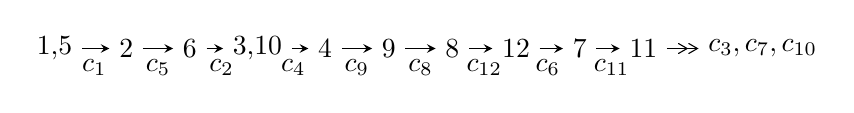
\begin{tikzpicture}[x=23pt, y=7pt]
	% node
	\node (A0) at (-1/8, 0) {1,5};
	\node (A1) at (1, 0) {2};
	\node (A2) at (2, 0) {6};
	\node (A3) at (49/16, 0) {3,10};
	\node (A4) at (33/8, 0) {4};
	\node (A5) at (41/8, 0) {9};
	\node (A6) at (49/8, 0) {8};
	\node (A7) at (57/8, 0) {12};
	\node (A8) at (65/8, 0) {7};
	\node (A9) at (73/8, 0) {11};
	\node (C1) at (1/2, -1) {$c_{1}$};
	\node (C2) at (3/2, -1) {$c_{5}$};
	\node (C3) at (5/2, -1) {$c_{2}$};
	\node (C4) at (29/8, -1) {$c_{4}$};
	\node (C5) at (37/8, -1) {$c_{9}$};
	\node (C6) at (45/8, -1) {$c_{8}$};
	\node (C7) at (53/8, -1) {$c_{12}$};
	\node (C8) at (61/8, -1) {$c_{6}$};
	\node (C9) at (69/8, -1) {$c_{11}$};
	\node (A10) at (11, 0) {$c_{3},c_{7},c_{10}$};

	% edge
	\draw[->,>=stealth]	
	(A0) edge (A1) (A1) edge (A2) (A2) edge (A3) (A3) edge (A4) (A4) edge (A5) (A5) edge (A6) (A6) edge (A7) (A7) edge (A8) (A8) edge (A9) ;
	\draw[->>,>={angle 60}]	
	(A9) edge (A10);
\end{tikzpicture} \\ 

\end{tabular} \\

\footnotetext{
The image of knot diagram is generated by the software ``\textbf{Draw programme}" developed by Andrew Bartholomew(\url{http://www.layer8.co.uk/maths/draw/index.htm\#Running-draw}), where we modified some parts for our purpose(\url{https://github.com/CATsTAILs/LinksPainter}).
}\phantom \\ \newline 
\centering \textbf{Ideals for irreducible components\footnotemark of $X_{\text{par}}$} 
 
\begin{align*}
I^u_{1}&=\langle 
1.21800\times10^{175} u^{86}+1.10072\times10^{176} u^{85}+\cdots+5.56542\times10^{175} b+9.38658\times10^{176},\\
\phantom{I^u_{1}}&\phantom{= \langle  }-2.03509\times10^{176} u^{86}+9.22272\times10^{176} u^{85}+\cdots+5.56542\times10^{175} a+3.49997\times10^{177},\\
\phantom{I^u_{1}}&\phantom{= \langle  }u^{87}-5 u^{86}+\cdots-31 u-1\rangle \\
I^u_{2}&=\langle 
3 u^{20}-5 u^{19}+\cdots+b-2,\;-3 u^{20}+4 u^{19}+\cdots+a+4,\;u^{21}-14 u^{19}+\cdots+u-1\rangle \\
I^u_{3}&=\langle 
b+1,\;- u^5+2 u^4+2 u^3-4 u^2+a- u+1,\;u^6-3 u^5+6 u^3-4 u^2+1\rangle \\
I^u_{4}&=\langle 
b+1,\;a-1,\;u+1\rangle \\
\\
\end{align*}
\raggedright * 4 irreducible components of $\dim_{\mathbb{C}}=0$, with total 115 representations.\\
\footnotetext{All coefficients of polynomials are rational numbers. But the coefficients are sometimes approximated in decimal forms when there is not enough margin.}
\newpage
\renewcommand{\arraystretch}{1}
\centering \section*{I. $I^u_{1}= \langle 1.22\times10^{175} u^{86}+1.10\times10^{176} u^{85}+\cdots+5.57\times10^{175} b+9.39\times10^{176},\;-2.04\times10^{176} u^{86}+9.22\times10^{176} u^{85}+\cdots+5.57\times10^{175} a+3.50\times10^{177},\;u^{87}-5 u^{86}+\cdots-31 u-1 \rangle$}
\flushleft \textbf{(i) Arc colorings}\\
\begin{tabular}{m{7pt} m{180pt} m{7pt} m{180pt} }
\flushright $a_{1}=$&$\begin{pmatrix}1\\0\end{pmatrix}$ \\
\flushright $a_{5}=$&$\begin{pmatrix}0\\u\end{pmatrix}$ \\
\flushright $a_{2}=$&$\begin{pmatrix}1\\u^2\end{pmatrix}$ \\
\flushright $a_{6}=$&$\begin{pmatrix}- u\\- u^3+u\end{pmatrix}$ \\
\flushright $a_{3}=$&$\begin{pmatrix}- u^2+1\\- u^4+2 u^2\end{pmatrix}$ \\
\flushright $a_{10}=$&$\begin{pmatrix}3.65668 u^{86}-16.5715 u^{85}+\cdots-1025.07 u-62.8879\\-0.218852 u^{86}-1.97778 u^{85}+\cdots-412.229 u-16.8659\end{pmatrix}$ \\
\flushright $a_{4}=$&$\begin{pmatrix}-20.1258 u^{86}+100.004 u^{85}+\cdots+3106.06 u+123.163\\1.01692 u^{86}-6.75872 u^{85}+\cdots-461.880 u-22.8410\end{pmatrix}$ \\
\flushright $a_{9}=$&$\begin{pmatrix}3.43783 u^{86}-18.5492 u^{85}+\cdots-1437.30 u-79.7538\\-0.218852 u^{86}-1.97778 u^{85}+\cdots-412.229 u-16.8659\end{pmatrix}$ \\
\flushright $a_{8}=$&$\begin{pmatrix}20.7323 u^{86}-106.664 u^{85}+\cdots-4060.99 u-176.355\\-1.96351 u^{86}+8.22272 u^{85}+\cdots+158.487 u+9.66986\end{pmatrix}$ \\
\flushright $a_{12}=$&$\begin{pmatrix}-21.5377 u^{86}+114.337 u^{85}+\cdots+5556.14 u+273.143\\1.30331 u^{86}-0.885320 u^{85}+\cdots+627.672 u+26.9509\end{pmatrix}$ \\
\flushright $a_{7}=$&$\begin{pmatrix}-3.73334 u^{86}+32.1426 u^{85}+\cdots+2150.24 u+65.7851\\8.70129 u^{86}-35.1065 u^{85}+\cdots-562.970 u-33.7329\end{pmatrix}$ \\
\flushright $a_{11}=$&$\begin{pmatrix}3.49067 u^{86}-18.8111 u^{85}+\cdots-1445.83 u-79.7310\\0.510581 u^{86}-4.63816 u^{85}+\cdots-407.668 u-16.8546\end{pmatrix}$\\&\end{tabular}
\flushleft \textbf{(ii) Obstruction class $= -1$}\\~\\
\flushleft \textbf{(iii) Cusp Shapes $= -3.04694 u^{86}+31.0771 u^{85}+\cdots+2704.70 u+109.774$}\\~\\
\newpage\renewcommand{\arraystretch}{1}
\flushleft \textbf{(iv) u-Polynomials at the component}\newline \\
\begin{tabular}{m{50pt}|m{274pt}}
Crossings & \hspace{64pt}u-Polynomials at each crossing \\
\hline $$\begin{aligned}c_{1},c_{2},c_{5}\end{aligned}$$&$\begin{aligned}
&u^{87}+5 u^{86}+\cdots-31 u+1
\end{aligned}$\\
\hline $$\begin{aligned}c_{3},c_{8}\end{aligned}$$&$\begin{aligned}
&u^{87}+2 u^{86}+\cdots+1867 u-1459
\end{aligned}$\\
\hline $$\begin{aligned}c_{4}\end{aligned}$$&$\begin{aligned}
&u^{87}- u^{86}+\cdots-108842 u+15817
\end{aligned}$\\
\hline $$\begin{aligned}c_{6},c_{7},c_{11}\end{aligned}$$&$\begin{aligned}
&u^{87}+2 u^{86}+\cdots-36 u+7
\end{aligned}$\\
\hline $$\begin{aligned}c_{9},c_{12}\end{aligned}$$&$\begin{aligned}
&u^{87}-9 u^{86}+\cdots+784 u-8
\end{aligned}$\\
\hline $$\begin{aligned}c_{10}\end{aligned}$$&$\begin{aligned}
&u^{87}+3 u^{86}+\cdots+619168 u+590297
\end{aligned}$\\
\hline
\end{tabular}\\~\\
\newpage\renewcommand{\arraystretch}{1}
\flushleft \textbf{(v) Riley Polynomials at the component}\newline \\
\begin{tabular}{m{50pt}|m{274pt}}
Crossings & \hspace{64pt}Riley Polynomials at each crossing \\
\hline $$\begin{aligned}c_{1},c_{2},c_{5}\end{aligned}$$&$\begin{aligned}
&y^{87}-91 y^{86}+\cdots+301 y-1
\end{aligned}$\\
\hline $$\begin{aligned}c_{3},c_{8}\end{aligned}$$&$\begin{aligned}
&y^{87}-64 y^{86}+\cdots+35213103 y-2128681
\end{aligned}$\\
\hline $$\begin{aligned}c_{4}\end{aligned}$$&$\begin{aligned}
&y^{87}+33 y^{86}+\cdots+197455366 y-250177489
\end{aligned}$\\
\hline $$\begin{aligned}c_{6},c_{7},c_{11}\end{aligned}$$&$\begin{aligned}
&y^{87}+90 y^{86}+\cdots+2206 y-49
\end{aligned}$\\
\hline $$\begin{aligned}c_{9},c_{12}\end{aligned}$$&$\begin{aligned}
&y^{87}-59 y^{86}+\cdots+638432 y-64
\end{aligned}$\\
\hline $$\begin{aligned}c_{10}\end{aligned}$$&$\begin{aligned}
&y^{87}-25 y^{86}+\cdots+7264616979632 y-348450548209
\end{aligned}$\\
\hline
\end{tabular}\\~\\
\newpage\flushleft \textbf{(vi) Complex Volumes and Cusp Shapes}
$$\begin{array}{c|c|c}  
\text{Solutions to }I^u_{1}& \I (\text{vol} + \sqrt{-1}CS) & \text{Cusp shape}\\
 \hline 
\begin{aligned}
u &= \phantom{-}0.919570 + 0.341269 I \\
a &= -0.230219 - 1.291490 I \\
b &= \phantom{-}1.018910 + 0.767688 I\end{aligned}
 & \phantom{-}4.92914 - 3.18573 I & \phantom{-0.000000 } 0 \\ \hline\begin{aligned}
u &= \phantom{-}0.919570 - 0.341269 I \\
a &= -0.230219 + 1.291490 I \\
b &= \phantom{-}1.018910 - 0.767688 I\end{aligned}
 & \phantom{-}4.92914 + 3.18573 I & \phantom{-0.000000 } 0 \\ \hline\begin{aligned}
u &= \phantom{-}0.643376 + 0.795200 I \\
a &= -0.443359 - 0.859364 I \\
b &= \phantom{-}1.129980 + 0.180708 I\end{aligned}
 & -3.41783 - 2.87585 I & \phantom{-0.000000 } 0 \\ \hline\begin{aligned}
u &= \phantom{-}0.643376 - 0.795200 I \\
a &= -0.443359 + 0.859364 I \\
b &= \phantom{-}1.129980 - 0.180708 I\end{aligned}
 & -3.41783 + 2.87585 I & \phantom{-0.000000 } 0 \\ \hline\begin{aligned}
u &= -0.801927 + 0.529130 I \\
a &= -1.221220 - 0.403028 I \\
b &= -0.518441 + 0.530723 I\end{aligned}
 & \phantom{-}8.78928 - 2.20079 I & \phantom{-0.000000 } 0 \\ \hline\begin{aligned}
u &= -0.801927 - 0.529130 I \\
a &= -1.221220 + 0.403028 I \\
b &= -0.518441 - 0.530723 I\end{aligned}
 & \phantom{-}8.78928 + 2.20079 I & \phantom{-0.000000 } 0 \\ \hline\begin{aligned}
u &= -0.605395 + 0.915337 I \\
a &= \phantom{-}0.449296 - 1.181010 I \\
b &= -1.230940 + 0.562762 I\end{aligned}
 & \phantom{-}6.97761 + 12.04090 I & \phantom{-0.000000 } 0 \\ \hline\begin{aligned}
u &= -0.605395 - 0.915337 I \\
a &= \phantom{-}0.449296 + 1.181010 I \\
b &= -1.230940 - 0.562762 I\end{aligned}
 & \phantom{-}6.97761 - 12.04090 I & \phantom{-0.000000 } 0 \\ \hline\begin{aligned}
u &= -0.524939 + 0.728503 I \\
a &= -0.50181 + 1.52469 I \\
b &= \phantom{-}1.221130 - 0.467400 I\end{aligned}
 & \phantom{-}0.17465 + 8.23740 I & \phantom{-0.000000 } 0 \\ \hline\begin{aligned}
u &= -0.524939 - 0.728503 I \\
a &= -0.50181 - 1.52469 I \\
b &= \phantom{-}1.221130 + 0.467400 I\end{aligned}
 & \phantom{-}0.17465 - 8.23740 I & \phantom{-0.000000 } 0\\
 \hline 
 \end{array}$$\newpage$$\begin{array}{c|c|c}  
\text{Solutions to }I^u_{1}& \I (\text{vol} + \sqrt{-1}CS) & \text{Cusp shape}\\
 \hline 
\begin{aligned}
u &= \phantom{-}1.146280 + 0.016740 I \\
a &= -0.218153 + 1.254070 I \\
b &= \phantom{-}0.883487 - 0.824717 I\end{aligned}
 & \phantom{-}5.16086 + 3.06951 I & \phantom{-0.000000 } 0 \\ \hline\begin{aligned}
u &= \phantom{-}1.146280 - 0.016740 I \\
a &= -0.218153 - 1.254070 I \\
b &= \phantom{-}0.883487 + 0.824717 I\end{aligned}
 & \phantom{-}5.16086 - 3.06951 I & \phantom{-0.000000 } 0 \\ \hline\begin{aligned}
u &= -0.421925 + 0.731310 I \\
a &= -0.889218 + 0.084686 I \\
b &= \phantom{-}1.110590 + 0.288943 I\end{aligned}
 & \phantom{-}0.35974 - 3.47491 I & \phantom{-0.000000 } 0 \\ \hline\begin{aligned}
u &= -0.421925 - 0.731310 I \\
a &= -0.889218 - 0.084686 I \\
b &= \phantom{-}1.110590 - 0.288943 I\end{aligned}
 & \phantom{-}0.35974 + 3.47491 I & \phantom{-0.000000 } 0 \\ \hline\begin{aligned}
u &= \phantom{-}0.073826 + 0.813368 I \\
a &= -1.60062 + 0.49196 I \\
b &= \phantom{-}0.899591 - 0.403821 I\end{aligned}
 & \phantom{-}7.79839 - 0.95510 I & \phantom{-0.000000 } 0 \\ \hline\begin{aligned}
u &= \phantom{-}0.073826 - 0.813368 I \\
a &= -1.60062 - 0.49196 I \\
b &= \phantom{-}0.899591 + 0.403821 I\end{aligned}
 & \phantom{-}7.79839 + 0.95510 I & \phantom{-0.000000 } 0 \\ \hline\begin{aligned}
u &= \phantom{-}1.20375\phantom{ +0.000000I} \\
a &= \phantom{-}0.466459\phantom{ +0.000000I} \\
b &= \phantom{-}0.00998561\phantom{ +0.000000I}\end{aligned}
 & -2.53324\phantom{ +0.000000I} & \phantom{-0.000000 } 0 \\ \hline\begin{aligned}
u &= -0.635177 + 1.044370 I \\
a &= \phantom{-}0.662353 - 0.064701 I \\
b &= -1.059810 - 0.347777 I\end{aligned}
 & \phantom{-}7.02919 - 5.71442 I & \phantom{-0.000000 } 0 \\ \hline\begin{aligned}
u &= -0.635177 - 1.044370 I \\
a &= \phantom{-}0.662353 + 0.064701 I \\
b &= -1.059810 + 0.347777 I\end{aligned}
 & \phantom{-}7.02919 + 5.71442 I & \phantom{-0.000000 } 0 \\ \hline\begin{aligned}
u &= \phantom{-}0.509200 + 1.127410 I \\
a &= \phantom{-}0.472655 + 0.551529 I \\
b &= -1.195790 - 0.258865 I\end{aligned}
 & \phantom{-}1.51094 - 5.10157 I & \phantom{-0.000000 } 0\\
 \hline 
 \end{array}$$\newpage$$\begin{array}{c|c|c}  
\text{Solutions to }I^u_{1}& \I (\text{vol} + \sqrt{-1}CS) & \text{Cusp shape}\\
 \hline 
\begin{aligned}
u &= \phantom{-}0.509200 - 1.127410 I \\
a &= \phantom{-}0.472655 - 0.551529 I \\
b &= -1.195790 + 0.258865 I\end{aligned}
 & \phantom{-}1.51094 + 5.10157 I & \phantom{-0.000000 } 0 \\ \hline\begin{aligned}
u &= -0.365776 + 0.653749 I \\
a &= -0.081284 + 1.401450 I \\
b &= -0.287242 - 1.062190 I\end{aligned}
 & \phantom{-}10.02620 + 6.30984 I & \phantom{-0.000000 } 0 \\ \hline\begin{aligned}
u &= -0.365776 - 0.653749 I \\
a &= -0.081284 - 1.401450 I \\
b &= -0.287242 + 1.062190 I\end{aligned}
 & \phantom{-}10.02620 - 6.30984 I & \phantom{-0.000000 } 0 \\ \hline\begin{aligned}
u &= \phantom{-}0.129351 + 0.704209 I \\
a &= -0.679190 - 0.828173 I \\
b &= \phantom{-}0.103762 + 0.686088 I\end{aligned}
 & \phantom{-}5.33081 - 1.86604 I & \phantom{-0.000000 -}0. + 3.90648 I \\ \hline\begin{aligned}
u &= \phantom{-}0.129351 - 0.704209 I \\
a &= -0.679190 + 0.828173 I \\
b &= \phantom{-}0.103762 - 0.686088 I\end{aligned}
 & \phantom{-}5.33081 + 1.86604 I & \phantom{-0.000000 } 0. - 3.90648 I \\ \hline\begin{aligned}
u &= \phantom{-}1.223970 + 0.401442 I \\
a &= -0.462473 - 0.267648 I \\
b &= -0.073035 - 0.139352 I\end{aligned}
 & \phantom{-}2.07456 - 2.27551 I & \phantom{-0.000000 } 0 \\ \hline\begin{aligned}
u &= \phantom{-}1.223970 - 0.401442 I \\
a &= -0.462473 + 0.267648 I \\
b &= -0.073035 + 0.139352 I\end{aligned}
 & \phantom{-}2.07456 + 2.27551 I & \phantom{-0.000000 } 0 \\ \hline\begin{aligned}
u &= -1.263230 + 0.374502 I \\
a &= -0.746639 + 0.577828 I \\
b &= \phantom{-}0.860702 + 0.092884 I\end{aligned}
 & \phantom{-}3.67205 + 5.24598 I & \phantom{-0.000000 } 0 \\ \hline\begin{aligned}
u &= -1.263230 - 0.374502 I \\
a &= -0.746639 - 0.577828 I \\
b &= \phantom{-}0.860702 - 0.092884 I\end{aligned}
 & \phantom{-}3.67205 - 5.24598 I & \phantom{-0.000000 } 0 \\ \hline\begin{aligned}
u &= -0.266580 + 0.588131 I \\
a &= \phantom{-}1.35207 - 2.09086 I \\
b &= -1.122390 + 0.353863 I\end{aligned}
 & \phantom{-}0.18453 + 2.81647 I & -0.56699 - 5.14375 I\\
 \hline 
 \end{array}$$\newpage$$\begin{array}{c|c|c}  
\text{Solutions to }I^u_{1}& \I (\text{vol} + \sqrt{-1}CS) & \text{Cusp shape}\\
 \hline 
\begin{aligned}
u &= -0.266580 - 0.588131 I \\
a &= \phantom{-}1.35207 + 2.09086 I \\
b &= -1.122390 - 0.353863 I\end{aligned}
 & \phantom{-}0.18453 - 2.81647 I & -0.56699 + 5.14375 I \\ \hline\begin{aligned}
u &= -0.383725 + 0.510780 I \\
a &= -0.35311 - 1.52762 I \\
b &= \phantom{-}0.127056 + 0.881304 I\end{aligned}
 & \phantom{-}3.55177 + 3.39819 I & \phantom{-}0.84018 - 6.92415 I \\ \hline\begin{aligned}
u &= -0.383725 - 0.510780 I \\
a &= -0.35311 + 1.52762 I \\
b &= \phantom{-}0.127056 - 0.881304 I\end{aligned}
 & \phantom{-}3.55177 - 3.39819 I & \phantom{-}0.84018 + 6.92415 I \\ \hline\begin{aligned}
u &= -0.631511\phantom{ +0.000000I} \\
a &= \phantom{-}0.479038\phantom{ +0.000000I} \\
b &= -1.15135\phantom{ +0.000000I}\end{aligned}
 & -1.55302\phantom{ +0.000000I} & -7.94170\phantom{ +0.000000I} \\ \hline\begin{aligned}
u &= \phantom{-}1.382990 + 0.055539 I \\
a &= \phantom{-}0.565031 - 0.732391 I \\
b &= -0.238430 + 0.708558 I\end{aligned}
 & -2.35948 - 0.82108 I & \phantom{-0.000000 } 0 \\ \hline\begin{aligned}
u &= \phantom{-}1.382990 - 0.055539 I \\
a &= \phantom{-}0.565031 + 0.732391 I \\
b &= -0.238430 - 0.708558 I\end{aligned}
 & -2.35948 + 0.82108 I & \phantom{-0.000000 } 0 \\ \hline\begin{aligned}
u &= -1.375540 + 0.190726 I \\
a &= \phantom{-}0.047286 + 0.731163 I \\
b &= \phantom{-}0.378703 - 1.174100 I\end{aligned}
 & \phantom{-}0.57233 + 4.93402 I & \phantom{-0.000000 } 0 \\ \hline\begin{aligned}
u &= -1.375540 - 0.190726 I \\
a &= \phantom{-}0.047286 - 0.731163 I \\
b &= \phantom{-}0.378703 + 1.174100 I\end{aligned}
 & \phantom{-}0.57233 - 4.93402 I & \phantom{-0.000000 } 0 \\ \hline\begin{aligned}
u &= -1.391300 + 0.009231 I \\
a &= \phantom{-}0.421080 + 0.806075 I \\
b &= \phantom{-}1.57036 - 0.71094 I\end{aligned}
 & -2.89241 + 2.70347 I & \phantom{-0.000000 } 0 \\ \hline\begin{aligned}
u &= -1.391300 - 0.009231 I \\
a &= \phantom{-}0.421080 - 0.806075 I \\
b &= \phantom{-}1.57036 + 0.71094 I\end{aligned}
 & -2.89241 - 2.70347 I & \phantom{-0.000000 } 0\\
 \hline 
 \end{array}$$\newpage$$\begin{array}{c|c|c}  
\text{Solutions to }I^u_{1}& \I (\text{vol} + \sqrt{-1}CS) & \text{Cusp shape}\\
 \hline 
\begin{aligned}
u &= -0.491766 + 0.337151 I \\
a &= \phantom{-}1.52671 + 1.10854 I \\
b &= \phantom{-}0.131068 - 0.467644 I\end{aligned}
 & \phantom{-}3.13228 - 0.27068 I & \phantom{-}1.77490 - 1.85357 I \\ \hline\begin{aligned}
u &= -0.491766 - 0.337151 I \\
a &= \phantom{-}1.52671 - 1.10854 I \\
b &= \phantom{-}0.131068 + 0.467644 I\end{aligned}
 & \phantom{-}3.13228 + 0.27068 I & \phantom{-}1.77490 + 1.85357 I \\ \hline\begin{aligned}
u &= -1.41338 + 0.09716 I \\
a &= \phantom{-}1.63265 - 0.41394 I \\
b &= \phantom{-}1.024190 - 0.080144 I\end{aligned}
 & \phantom{-}3.14701 + 6.03465 I & \phantom{-0.000000 } 0 \\ \hline\begin{aligned}
u &= -1.41338 - 0.09716 I \\
a &= \phantom{-}1.63265 + 0.41394 I \\
b &= \phantom{-}1.024190 + 0.080144 I\end{aligned}
 & \phantom{-}3.14701 - 6.03465 I & \phantom{-0.000000 } 0 \\ \hline\begin{aligned}
u &= \phantom{-}1.42796 + 0.02959 I \\
a &= \phantom{-}0.701919 + 0.520870 I \\
b &= \phantom{-}1.53124 - 0.11552 I\end{aligned}
 & -3.60289 - 2.95271 I & \phantom{-0.000000 } 0 \\ \hline\begin{aligned}
u &= \phantom{-}1.42796 - 0.02959 I \\
a &= \phantom{-}0.701919 - 0.520870 I \\
b &= \phantom{-}1.53124 + 0.11552 I\end{aligned}
 & -3.60289 + 2.95271 I & \phantom{-0.000000 } 0 \\ \hline\begin{aligned}
u &= -1.43990 + 0.06670 I \\
a &= -0.012806 - 0.753944 I \\
b &= -0.183222 + 0.885034 I\end{aligned}
 & -5.79294 + 2.10750 I & \phantom{-0.000000 } 0 \\ \hline\begin{aligned}
u &= -1.43990 - 0.06670 I \\
a &= -0.012806 + 0.753944 I \\
b &= -0.183222 - 0.885034 I\end{aligned}
 & -5.79294 - 2.10750 I & \phantom{-0.000000 } 0 \\ \hline\begin{aligned}
u &= \phantom{-}1.43586 + 0.20746 I \\
a &= -0.41468 + 1.49380 I \\
b &= -1.226660 - 0.529473 I\end{aligned}
 & -5.35379 - 5.68624 I & \phantom{-0.000000 } 0 \\ \hline\begin{aligned}
u &= \phantom{-}1.43586 - 0.20746 I \\
a &= -0.41468 - 1.49380 I \\
b &= -1.226660 + 0.529473 I\end{aligned}
 & -5.35379 + 5.68624 I & \phantom{-0.000000 } 0\\
 \hline 
 \end{array}$$\newpage$$\begin{array}{c|c|c}  
\text{Solutions to }I^u_{1}& \I (\text{vol} + \sqrt{-1}CS) & \text{Cusp shape}\\
 \hline 
\begin{aligned}
u &= \phantom{-}1.45502 + 0.14563 I \\
a &= -0.310433 + 0.637258 I \\
b &= \phantom{-}0.052332 - 1.193180 I\end{aligned}
 & -2.41136 - 5.70802 I & \phantom{-0.000000 } 0 \\ \hline\begin{aligned}
u &= \phantom{-}1.45502 - 0.14563 I \\
a &= -0.310433 - 0.637258 I \\
b &= \phantom{-}0.052332 + 1.193180 I\end{aligned}
 & -2.41136 + 5.70802 I & \phantom{-0.000000 } 0 \\ \hline\begin{aligned}
u &= \phantom{-}0.427368 + 0.306228 I \\
a &= \phantom{-}0.86564 + 1.62484 I \\
b &= -1.109570 - 0.540320 I\end{aligned}
 & -1.27209 - 2.61374 I & -8.1476 + 11.5732 I \\ \hline\begin{aligned}
u &= \phantom{-}0.427368 - 0.306228 I \\
a &= \phantom{-}0.86564 - 1.62484 I \\
b &= -1.109570 + 0.540320 I\end{aligned}
 & -1.27209 + 2.61374 I & -8.1476 - 11.5732 I \\ \hline\begin{aligned}
u &= \phantom{-}1.47311 + 0.21321 I \\
a &= \phantom{-}0.208305 - 0.640823 I \\
b &= -0.17007 + 1.45424 I\end{aligned}
 & \phantom{-}4.02421 - 9.40391 I & \phantom{-0.000000 } 0 \\ \hline\begin{aligned}
u &= \phantom{-}1.47311 - 0.21321 I \\
a &= \phantom{-}0.208305 + 0.640823 I \\
b &= -0.17007 - 1.45424 I\end{aligned}
 & \phantom{-}4.02421 + 9.40391 I & \phantom{-0.000000 } 0 \\ \hline\begin{aligned}
u &= \phantom{-}1.49510 + 0.04344 I \\
a &= -0.581323 + 0.412900 I \\
b &= -1.51105 - 0.29367 I\end{aligned}
 & -8.12584 - 0.44534 I & \phantom{-0.000000 } 0 \\ \hline\begin{aligned}
u &= \phantom{-}1.49510 - 0.04344 I \\
a &= -0.581323 - 0.412900 I \\
b &= -1.51105 + 0.29367 I\end{aligned}
 & -8.12584 + 0.44534 I & \phantom{-0.000000 } 0 \\ \hline\begin{aligned}
u &= -0.469577 + 0.132148 I \\
a &= \phantom{-}0.607127 + 0.383204 I \\
b &= \phantom{-}1.022440 - 0.664659 I\end{aligned}
 & \phantom{-}2.30869 + 3.10979 I & \phantom{-}6.28767 + 0.10476 I \\ \hline\begin{aligned}
u &= -0.469577 - 0.132148 I \\
a &= \phantom{-}0.607127 - 0.383204 I \\
b &= \phantom{-}1.022440 + 0.664659 I\end{aligned}
 & \phantom{-}2.30869 - 3.10979 I & \phantom{-}6.28767 - 0.10476 I\\
 \hline 
 \end{array}$$\newpage$$\begin{array}{c|c|c}  
\text{Solutions to }I^u_{1}& \I (\text{vol} + \sqrt{-1}CS) & \text{Cusp shape}\\
 \hline 
\begin{aligned}
u &= -1.51638 + 0.07781 I \\
a &= -0.311568 - 0.786453 I \\
b &= -1.38732 + 0.85466 I\end{aligned}
 & -7.83146 + 3.89655 I & \phantom{-0.000000 } 0 \\ \hline\begin{aligned}
u &= -1.51638 - 0.07781 I \\
a &= -0.311568 + 0.786453 I \\
b &= -1.38732 - 0.85466 I\end{aligned}
 & -7.83146 - 3.89655 I & \phantom{-0.000000 } 0 \\ \hline\begin{aligned}
u &= \phantom{-}1.54839 + 0.05770 I \\
a &= \phantom{-}0.443126 - 0.341427 I \\
b &= \phantom{-}1.47115 + 0.67450 I\end{aligned}
 & -4.62587 - 3.85006 I & \phantom{-0.000000 } 0 \\ \hline\begin{aligned}
u &= \phantom{-}1.54839 - 0.05770 I \\
a &= \phantom{-}0.443126 + 0.341427 I \\
b &= \phantom{-}1.47115 - 0.67450 I\end{aligned}
 & -4.62587 + 3.85006 I & \phantom{-0.000000 } 0 \\ \hline\begin{aligned}
u &= \phantom{-}1.52731 + 0.26111 I \\
a &= \phantom{-}0.475990 - 1.199960 I \\
b &= \phantom{-}1.36229 + 0.58251 I\end{aligned}
 & -6.51610 - 11.88980 I & \phantom{-0.000000 } 0 \\ \hline\begin{aligned}
u &= \phantom{-}1.52731 - 0.26111 I \\
a &= \phantom{-}0.475990 + 1.199960 I \\
b &= \phantom{-}1.36229 - 0.58251 I\end{aligned}
 & -6.51610 + 11.88980 I & \phantom{-0.000000 } 0 \\ \hline\begin{aligned}
u &= -1.54118 + 0.17061 I \\
a &= -0.318296 - 1.038990 I \\
b &= -1.170070 + 0.386041 I\end{aligned}
 & -8.66512 + 2.45063 I & \phantom{-0.000000 } 0 \\ \hline\begin{aligned}
u &= -1.54118 - 0.17061 I \\
a &= -0.318296 + 1.038990 I \\
b &= -1.170070 - 0.386041 I\end{aligned}
 & -8.66512 - 2.45063 I & \phantom{-0.000000 } 0 \\ \hline\begin{aligned}
u &= \phantom{-}0.277564 + 0.317493 I \\
a &= \phantom{-}0.560535 + 1.041500 I \\
b &= -0.079901 - 0.308666 I\end{aligned}
 & -0.183792 - 0.864472 I & -4.29913 + 7.86972 I \\ \hline\begin{aligned}
u &= \phantom{-}0.277564 - 0.317493 I \\
a &= \phantom{-}0.560535 - 1.041500 I \\
b &= -0.079901 + 0.308666 I\end{aligned}
 & -0.183792 + 0.864472 I & -4.29913 - 7.86972 I\\
 \hline 
 \end{array}$$\newpage$$\begin{array}{c|c|c}  
\text{Solutions to }I^u_{1}& \I (\text{vol} + \sqrt{-1}CS) & \text{Cusp shape}\\
 \hline 
\begin{aligned}
u &= -1.56054 + 0.25243 I \\
a &= \phantom{-}0.375410 + 0.928178 I \\
b &= \phantom{-}1.353380 - 0.393780 I\end{aligned}
 & -10.60940 + 6.66212 I & \phantom{-0.000000 } 0 \\ \hline\begin{aligned}
u &= -1.56054 - 0.25243 I \\
a &= \phantom{-}0.375410 - 0.928178 I \\
b &= \phantom{-}1.353380 + 0.393780 I\end{aligned}
 & -10.60940 - 6.66212 I & \phantom{-0.000000 } 0 \\ \hline\begin{aligned}
u &= -1.55851 + 0.35179 I \\
a &= -0.349517 - 0.886182 I \\
b &= -1.44084 + 0.41048 I\end{aligned}
 & -5.19961 + 10.21640 I & \phantom{-0.000000 } 0 \\ \hline\begin{aligned}
u &= -1.55851 - 0.35179 I \\
a &= -0.349517 + 0.886182 I \\
b &= -1.44084 - 0.41048 I\end{aligned}
 & -5.19961 - 10.21640 I & \phantom{-0.000000 } 0 \\ \hline\begin{aligned}
u &= \phantom{-}1.57773 + 0.32081 I \\
a &= -0.413286 + 1.072970 I \\
b &= -1.42145 - 0.65571 I\end{aligned}
 & -0.1084 - 16.5867 I & \phantom{-0.000000 } 0 \\ \hline\begin{aligned}
u &= \phantom{-}1.57773 - 0.32081 I \\
a &= -0.413286 - 1.072970 I \\
b &= -1.42145 + 0.65571 I\end{aligned}
 & -0.1084 + 16.5867 I & \phantom{-0.000000 } 0 \\ \hline\begin{aligned}
u &= -1.60922 + 0.08030 I \\
a &= \phantom{-}0.270773 + 0.717828 I \\
b &= \phantom{-}1.37271 - 1.07445 I\end{aligned}
 & -3.46237 + 4.60398 I & \phantom{-0.000000 } 0 \\ \hline\begin{aligned}
u &= -1.60922 - 0.08030 I \\
a &= \phantom{-}0.270773 - 0.717828 I \\
b &= \phantom{-}1.37271 + 1.07445 I\end{aligned}
 & -3.46237 - 4.60398 I & \phantom{-0.000000 } 0 \\ \hline\begin{aligned}
u &= \phantom{-}0.125878 + 0.322657 I \\
a &= \phantom{-}3.80205 - 2.84036 I \\
b &= \phantom{-}0.779351 + 0.457129 I\end{aligned}
 & \phantom{-}8.28711 - 4.58904 I & \phantom{-}1.66459 + 8.40382 I \\ \hline\begin{aligned}
u &= \phantom{-}0.125878 - 0.322657 I \\
a &= \phantom{-}3.80205 + 2.84036 I \\
b &= \phantom{-}0.779351 - 0.457129 I\end{aligned}
 & \phantom{-}8.28711 + 4.58904 I & \phantom{-}1.66459 - 8.40382 I\\
 \hline 
 \end{array}$$\newpage$$\begin{array}{c|c|c}  
\text{Solutions to }I^u_{1}& \I (\text{vol} + \sqrt{-1}CS) & \text{Cusp shape}\\
 \hline 
\begin{aligned}
u &= \phantom{-}1.55309 + 0.60898 I \\
a &= -0.171676 + 0.555702 I \\
b &= -1.234490 - 0.047231 I\end{aligned}
 & -1.64260 - 2.30540 I & \phantom{-0.000000 } 0 \\ \hline\begin{aligned}
u &= \phantom{-}1.55309 - 0.60898 I \\
a &= -0.171676 - 0.555702 I \\
b &= -1.234490 + 0.047231 I\end{aligned}
 & -1.64260 + 2.30540 I & \phantom{-0.000000 } 0 \\ \hline\begin{aligned}
u &= \phantom{-}1.64697 + 0.30699 I \\
a &= \phantom{-}0.307607 - 0.488246 I \\
b &= \phantom{-}1.146860 + 0.090509 I\end{aligned}
 & -6.04528 - 1.09420 I & \phantom{-0.000000 } 0 \\ \hline\begin{aligned}
u &= \phantom{-}1.64697 - 0.30699 I \\
a &= \phantom{-}0.307607 + 0.488246 I \\
b &= \phantom{-}1.146860 - 0.090509 I\end{aligned}
 & -6.04528 + 1.09420 I & \phantom{-0.000000 } 0 \\ \hline\begin{aligned}
u &= -0.124790\phantom{ +0.000000I} \\
a &= \phantom{-}13.9437\phantom{ +0.000000I} \\
b &= -0.470722\phantom{ +0.000000I}\end{aligned}
 & \phantom{-}2.89659\phantom{ +0.000000I} & \phantom{-}10.5150\phantom{ +0.000000I} \\ \hline\begin{aligned}
u &= -0.0876446 + 0.0176727 I \\
a &= \phantom{-}2.61863 - 7.91258 I \\
b &= \phantom{-}1.41551 - 0.34649 I\end{aligned}
 & \phantom{-}1.67209 + 2.65200 I & -6.68294 + 0.54441 I \\ \hline\begin{aligned}
u &= -0.0876446 - 0.0176727 I \\
a &= \phantom{-}2.61863 + 7.91258 I \\
b &= \phantom{-}1.41551 + 0.34649 I\end{aligned}
 & \phantom{-}1.67209 - 2.65200 I & -6.68294 - 0.54441 I\\
 \hline 
 \end{array}$$\newpage\newpage\renewcommand{\arraystretch}{1}
\centering \section*{II. $I^u_{2}= \langle 3 u^{20}-5 u^{19}+\cdots+b-2,\;-3 u^{20}+4 u^{19}+\cdots+a+4,\;u^{21}-14 u^{19}+\cdots+u-1 \rangle$}
\flushleft \textbf{(i) Arc colorings}\\
\begin{tabular}{m{7pt} m{180pt} m{7pt} m{180pt} }
\flushright $a_{1}=$&$\begin{pmatrix}1\\0\end{pmatrix}$ \\
\flushright $a_{5}=$&$\begin{pmatrix}0\\u\end{pmatrix}$ \\
\flushright $a_{2}=$&$\begin{pmatrix}1\\u^2\end{pmatrix}$ \\
\flushright $a_{6}=$&$\begin{pmatrix}- u\\- u^3+u\end{pmatrix}$ \\
\flushright $a_{3}=$&$\begin{pmatrix}- u^2+1\\- u^4+2 u^2\end{pmatrix}$ \\
\flushright $a_{10}=$&$\begin{pmatrix}3 u^{20}-4 u^{19}+\cdots+12 u-4\\-3 u^{20}+5 u^{19}+\cdots-4 u+2\end{pmatrix}$ \\
\flushright $a_{4}=$&$\begin{pmatrix}u^{20}-2 u^{19}+\cdots-4 u+3\\-4 u^{20}+5 u^{19}+\cdots-5 u+2\end{pmatrix}$ \\
\flushright $a_{9}=$&$\begin{pmatrix}u^{19}-3 u^{18}+\cdots+8 u-2\\-3 u^{20}+5 u^{19}+\cdots-4 u+2\end{pmatrix}$ \\
\flushright $a_{8}=$&$\begin{pmatrix}-3 u^{20}+3 u^{19}+\cdots-7 u+5\\u^{20}- u^{19}+\cdots+2 u-2\end{pmatrix}$ \\
\flushright $a_{12}=$&$\begin{pmatrix}2 u^{20}-3 u^{19}+\cdots+8 u-3\\u^{19}- u^{18}+\cdots-5 u^2-2 u\end{pmatrix}$ \\
\flushright $a_{7}=$&$\begin{pmatrix}-3 u^{20}+4 u^{19}+\cdots-4 u+3\\- u^{20}+3 u^{19}+\cdots- u+1\end{pmatrix}$ \\
\flushright $a_{11}=$&$\begin{pmatrix}-2 u^{20}+4 u^{19}+\cdots-5 u^2+5 u\\-7 u^{20}+10 u^{19}+\cdots-9 u+5\end{pmatrix}$\\&\end{tabular}
\flushleft \textbf{(ii) Obstruction class $= 1$}\\~\\
\flushleft \textbf{(iii) Cusp Shapes $= 7 u^{20}-13 u^{19}-84 u^{18}+158 u^{17}+425 u^{16}-809 u^{15}-1168 u^{14}+2256 u^{13}+1870 u^{12}-3697 u^{11}-1742 u^{10}+3586 u^9+919 u^8-1994 u^7-306 u^6+636 u^5+87 u^4-158 u^3+7 u^2+24 u-16$}\\~\\
\newpage\renewcommand{\arraystretch}{1}
\flushleft \textbf{(iv) u-Polynomials at the component}\newline \\
\begin{tabular}{m{50pt}|m{274pt}}
Crossings & \hspace{64pt}u-Polynomials at each crossing \\
\hline $$\begin{aligned}c_{1},c_{2}\end{aligned}$$&$\begin{aligned}
&u^{21}-14 u^{19}+\cdots+u-1
\end{aligned}$\\
\hline $$\begin{aligned}c_{3}\end{aligned}$$&$\begin{aligned}
&u^{21}+u^{20}+\cdots- u+1
\end{aligned}$\\
\hline $$\begin{aligned}c_{4}\end{aligned}$$&$\begin{aligned}
&u^{21}-2 u^{19}+\cdots-2 u-1
\end{aligned}$\\
\hline $$\begin{aligned}c_{5}\end{aligned}$$&$\begin{aligned}
&u^{21}-14 u^{19}+\cdots+u+1
\end{aligned}$\\
\hline $$\begin{aligned}c_{6},c_{7}\end{aligned}$$&$\begin{aligned}
&u^{21}+u^{20}+\cdots-9 u^2-1
\end{aligned}$\\
\hline $$\begin{aligned}c_{8}\end{aligned}$$&$\begin{aligned}
&u^{21}- u^{20}+\cdots- u-1
\end{aligned}$\\
\hline $$\begin{aligned}c_{9}\end{aligned}$$&$\begin{aligned}
&u^{21}+3 u^{20}+\cdots+9 u^2-1
\end{aligned}$\\
\hline $$\begin{aligned}c_{10}\end{aligned}$$&$\begin{aligned}
&u^{21}+3 u^{19}+\cdots-8 u^2+1
\end{aligned}$\\
\hline $$\begin{aligned}c_{11}\end{aligned}$$&$\begin{aligned}
&u^{21}- u^{20}+\cdots+9 u^2+1
\end{aligned}$\\
\hline $$\begin{aligned}c_{12}\end{aligned}$$&$\begin{aligned}
&u^{21}-3 u^{20}+\cdots-9 u^2+1
\end{aligned}$\\
\hline
\end{tabular}\\~\\
\newpage\renewcommand{\arraystretch}{1}
\flushleft \textbf{(v) Riley Polynomials at the component}\newline \\
\begin{tabular}{m{50pt}|m{274pt}}
Crossings & \hspace{64pt}Riley Polynomials at each crossing \\
\hline $$\begin{aligned}c_{1},c_{2},c_{5}\end{aligned}$$&$\begin{aligned}
&y^{21}-28 y^{20}+\cdots+9 y-1
\end{aligned}$\\
\hline $$\begin{aligned}c_{3},c_{8}\end{aligned}$$&$\begin{aligned}
&y^{21}-21 y^{20}+\cdots+11 y-1
\end{aligned}$\\
\hline $$\begin{aligned}c_{4}\end{aligned}$$&$\begin{aligned}
&y^{21}-4 y^{20}+\cdots-10 y-1
\end{aligned}$\\
\hline $$\begin{aligned}c_{6},c_{7},c_{11}\end{aligned}$$&$\begin{aligned}
&y^{21}+21 y^{20}+\cdots-18 y-1
\end{aligned}$\\
\hline $$\begin{aligned}c_{9},c_{12}\end{aligned}$$&$\begin{aligned}
&y^{21}-17 y^{20}+\cdots+18 y-1
\end{aligned}$\\
\hline $$\begin{aligned}c_{10}\end{aligned}$$&$\begin{aligned}
&y^{21}+6 y^{20}+\cdots+16 y-1
\end{aligned}$\\
\hline
\end{tabular}\\~\\
\newpage\flushleft \textbf{(vi) Complex Volumes and Cusp Shapes}
$$\begin{array}{c|c|c}  
\text{Solutions to }I^u_{2}& \I (\text{vol} + \sqrt{-1}CS) & \text{Cusp shape}\\
 \hline 
\begin{aligned}
u &= \phantom{-}0.980123 + 0.287889 I \\
a &= -0.202219 - 0.402737 I \\
b &= \phantom{-}0.821250 + 0.530110 I\end{aligned}
 & \phantom{-}1.64253 - 3.32447 I & -6.73227 + 3.23371 I \\ \hline\begin{aligned}
u &= \phantom{-}0.980123 - 0.287889 I \\
a &= -0.202219 + 0.402737 I \\
b &= \phantom{-}0.821250 - 0.530110 I\end{aligned}
 & \phantom{-}1.64253 + 3.32447 I & -6.73227 - 3.23371 I \\ \hline\begin{aligned}
u &= \phantom{-}1.12877\phantom{ +0.000000I} \\
a &= \phantom{-}0.459570\phantom{ +0.000000I} \\
b &= -0.644952\phantom{ +0.000000I}\end{aligned}
 & -3.11468\phantom{ +0.000000I} & -14.6860\phantom{ +0.000000I} \\ \hline\begin{aligned}
u &= -1.23262\phantom{ +0.000000I} \\
a &= \phantom{-}1.72801\phantom{ +0.000000I} \\
b &= -0.411550\phantom{ +0.000000I}\end{aligned}
 & -0.191889\phantom{ +0.000000I} & \phantom{-}1.35120\phantom{ +0.000000I} \\ \hline\begin{aligned}
u &= -1.267400 + 0.189837 I \\
a &= -1.145350 + 0.468508 I \\
b &= \phantom{-}0.372541 - 0.430174 I\end{aligned}
 & \phantom{-}5.01252 + 5.95890 I & \phantom{-}0.38975 - 5.02691 I \\ \hline\begin{aligned}
u &= -1.267400 - 0.189837 I \\
a &= -1.145350 - 0.468508 I \\
b &= \phantom{-}0.372541 + 0.430174 I\end{aligned}
 & \phantom{-}5.01252 - 5.95890 I & \phantom{-}0.38975 + 5.02691 I \\ \hline\begin{aligned}
u &= \phantom{-}0.513299 + 0.356158 I \\
a &= -0.298859 - 0.889580 I \\
b &= \phantom{-}1.198820 + 0.616343 I\end{aligned}
 & \phantom{-}1.84979 - 3.43907 I & -5.77787 + 8.99517 I \\ \hline\begin{aligned}
u &= \phantom{-}0.513299 - 0.356158 I \\
a &= -0.298859 + 0.889580 I \\
b &= \phantom{-}1.198820 - 0.616343 I\end{aligned}
 & \phantom{-}1.84979 + 3.43907 I & -5.77787 - 8.99517 I \\ \hline\begin{aligned}
u &= -0.428378 + 0.445644 I \\
a &= \phantom{-}0.59208 + 1.78035 I \\
b &= \phantom{-}0.635250 + 0.374830 I\end{aligned}
 & \phantom{-}8.00683 - 3.75384 I & -1.41538 + 0.52564 I \\ \hline\begin{aligned}
u &= -0.428378 - 0.445644 I \\
a &= \phantom{-}0.59208 - 1.78035 I \\
b &= \phantom{-}0.635250 - 0.374830 I\end{aligned}
 & \phantom{-}8.00683 + 3.75384 I & -1.41538 - 0.52564 I\\
 \hline 
 \end{array}$$\newpage$$\begin{array}{c|c|c}  
\text{Solutions to }I^u_{2}& \I (\text{vol} + \sqrt{-1}CS) & \text{Cusp shape}\\
 \hline 
\begin{aligned}
u &= -1.50488 + 0.09457 I \\
a &= -0.300529 - 0.973392 I \\
b &= -1.25356 + 0.73428 I\end{aligned}
 & -7.16310 + 3.43030 I & -3.74353 - 1.15763 I \\ \hline\begin{aligned}
u &= -1.50488 - 0.09457 I \\
a &= -0.300529 + 0.973392 I \\
b &= -1.25356 - 0.73428 I\end{aligned}
 & -7.16310 - 3.43030 I & -3.74353 + 1.15763 I \\ \hline\begin{aligned}
u &= -1.54873 + 0.07946 I \\
a &= \phantom{-}0.337710 + 0.596656 I \\
b &= \phantom{-}1.56117 - 0.99590 I\end{aligned}
 & -5.11343 + 4.80864 I & -8.81380 - 6.84118 I \\ \hline\begin{aligned}
u &= -1.54873 - 0.07946 I \\
a &= \phantom{-}0.337710 - 0.596656 I \\
b &= \phantom{-}1.56117 + 0.99590 I\end{aligned}
 & -5.11343 - 4.80864 I & -8.81380 + 6.84118 I \\ \hline\begin{aligned}
u &= -0.428907\phantom{ +0.000000I} \\
a &= -3.99233\phantom{ +0.000000I} \\
b &= -0.611834\phantom{ +0.000000I}\end{aligned}
 & \phantom{-}2.58386\phantom{ +0.000000I} & -16.1200\phantom{ +0.000000I} \\ \hline\begin{aligned}
u &= \phantom{-}1.55858 + 0.20556 I \\
a &= -0.410534 + 0.603726 I \\
b &= -1.123510 - 0.131583 I\end{aligned}
 & -5.66515 - 0.90405 I & -2.75648 - 2.17520 I \\ \hline\begin{aligned}
u &= \phantom{-}1.55858 - 0.20556 I \\
a &= -0.410534 - 0.603726 I \\
b &= -1.123510 + 0.131583 I\end{aligned}
 & -5.66515 + 0.90405 I & -2.75648 + 2.17520 I \\ \hline\begin{aligned}
u &= \phantom{-}0.213126 + 0.328797 I \\
a &= \phantom{-}2.06155 + 1.99092 I \\
b &= -1.118860 - 0.369484 I\end{aligned}
 & -1.13219 - 1.99292 I & -5.58755 - 0.19985 I \\ \hline\begin{aligned}
u &= \phantom{-}0.213126 - 0.328797 I \\
a &= \phantom{-}2.06155 - 1.99092 I \\
b &= -1.118860 + 0.369484 I\end{aligned}
 & -1.13219 + 1.99292 I & -5.58755 + 0.19985 I \\ \hline\begin{aligned}
u &= \phantom{-}1.75063 + 0.30855 I \\
a &= \phantom{-}0.268529 - 0.284726 I \\
b &= \phantom{-}1.241070 + 0.159795 I\end{aligned}
 & -2.01124 - 1.49085 I & -8.33532 + 1.09996 I\\
 \hline 
 \end{array}$$\newpage$$\begin{array}{c|c|c}  
\text{Solutions to }I^u_{2}& \I (\text{vol} + \sqrt{-1}CS) & \text{Cusp shape}\\
 \hline 
\begin{aligned}
u &= \phantom{-}1.75063 - 0.30855 I \\
a &= \phantom{-}0.268529 + 0.284726 I \\
b &= \phantom{-}1.241070 - 0.159795 I\end{aligned}
 & -2.01124 + 1.49085 I & -8.33532 - 1.09996 I\\
 \hline 
 \end{array}$$\newpage\newpage\renewcommand{\arraystretch}{1}
\centering \section*{III. $I^u_{3}= \langle b+1,\;- u^5+2 u^4+2 u^3-4 u^2+a- u+1,\;u^6-3 u^5+6 u^3-4 u^2+1 \rangle$}
\flushleft \textbf{(i) Arc colorings}\\
\begin{tabular}{m{7pt} m{180pt} m{7pt} m{180pt} }
\flushright $a_{1}=$&$\begin{pmatrix}1\\0\end{pmatrix}$ \\
\flushright $a_{5}=$&$\begin{pmatrix}0\\u\end{pmatrix}$ \\
\flushright $a_{2}=$&$\begin{pmatrix}1\\u^2\end{pmatrix}$ \\
\flushright $a_{6}=$&$\begin{pmatrix}- u\\- u^3+u\end{pmatrix}$ \\
\flushright $a_{3}=$&$\begin{pmatrix}- u^2+1\\- u^4+2 u^2\end{pmatrix}$ \\
\flushright $a_{10}=$&$\begin{pmatrix}u^5-2 u^4-2 u^3+4 u^2+u-1\\-1\end{pmatrix}$ \\
\flushright $a_{4}=$&$\begin{pmatrix}u^4-2 u^3- u^2+2 u+1\\u^5-2 u^4-2 u^3+5 u^2-1\end{pmatrix}$ \\
\flushright $a_{9}=$&$\begin{pmatrix}u^5-2 u^4-2 u^3+4 u^2+u-2\\-1\end{pmatrix}$ \\
\flushright $a_{8}=$&$\begin{pmatrix}- u^3+2 u^2-2\\- u^5+2 u^4+u^3-4 u^2+u\end{pmatrix}$ \\
\flushright $a_{12}=$&$\begin{pmatrix}u^5-2 u^4-2 u^3+4 u^2+u-1\\-1\end{pmatrix}$ \\
\flushright $a_{7}=$&$\begin{pmatrix}- u^2+1\\- u^4+2 u^2\end{pmatrix}$ \\
\flushright $a_{11}=$&$\begin{pmatrix}- u^5+u^4+2 u^3-2 u^2+2 u\\-3 u^5+4 u^4+6 u^3-7 u^2+2 u+1\end{pmatrix}$\\&\end{tabular}
\flushleft \textbf{(ii) Obstruction class $= -1$}\\~\\
\flushleft \textbf{(iii) Cusp Shapes $= -6$}\\~\\
\newpage\renewcommand{\arraystretch}{1}
\flushleft \textbf{(iv) u-Polynomials at the component}\newline \\
\begin{tabular}{m{50pt}|m{274pt}}
Crossings & \hspace{64pt}u-Polynomials at each crossing \\
\hline $$\begin{aligned}c_{1},c_{2},c_{5}\end{aligned}$$&$\begin{aligned}
&u^6+3 u^5-6 u^3-4 u^2+1
\end{aligned}$\\
\hline $$\begin{aligned}c_{3},c_{8}\end{aligned}$$&$\begin{aligned}
&u^6-3 u^5+6 u^3-4 u^2+1
\end{aligned}$\\
\hline $$\begin{aligned}c_{4}\end{aligned}$$&$\begin{aligned}
&u^6+u^5-2 u^4+6 u^3-4 u^2+2 u+1
\end{aligned}$\\
\hline $$\begin{aligned}c_{6},c_{7},c_{10}\\c_{11}\end{aligned}$$&$\begin{aligned}
&u^6- u^5+2 u^4-2 u^3-1
\end{aligned}$\\
\hline $$\begin{aligned}c_{9},c_{12}\end{aligned}$$&$\begin{aligned}
&(u+1)^6
\end{aligned}$\\
\hline
\end{tabular}\\~\\
\newpage\renewcommand{\arraystretch}{1}
\flushleft \textbf{(v) Riley Polynomials at the component}\newline \\
\begin{tabular}{m{50pt}|m{274pt}}
Crossings & \hspace{64pt}Riley Polynomials at each crossing \\
\hline $$\begin{aligned}c_{1},c_{2},c_{3}\\c_{5},c_{8}\end{aligned}$$&$\begin{aligned}
&y^6-9 y^5+28 y^4-34 y^3+16 y^2-8 y+1
\end{aligned}$\\
\hline $$\begin{aligned}c_{4}\end{aligned}$$&$\begin{aligned}
&y^6-5 y^5-16 y^4-22 y^3-12 y^2-12 y+1
\end{aligned}$\\
\hline $$\begin{aligned}c_{6},c_{7},c_{10}\\c_{11}\end{aligned}$$&$\begin{aligned}
&y^6+3 y^5-6 y^3-4 y^2+1
\end{aligned}$\\
\hline $$\begin{aligned}c_{9},c_{12}\end{aligned}$$&$\begin{aligned}
&(y-1)^6
\end{aligned}$\\
\hline
\end{tabular}\\~\\
\newpage\flushleft \textbf{(vi) Complex Volumes and Cusp Shapes}
$$\begin{array}{c|c|c}  
\text{Solutions to }I^u_{3}& \I (\text{vol} + \sqrt{-1}CS) & \text{Cusp shape}\\
 \hline 
\begin{aligned}
u &= \phantom{-}0.558227 + 0.461646 I \\
a &= \phantom{-}0.64026 + 1.59235 I \\
b &= -1.00000\phantom{ +0.000000I}\end{aligned}
 & -1.64493\phantom{ +0.000000I} & -6.00000\phantom{ +0.000000I} \\ \hline\begin{aligned}
u &= \phantom{-}0.558227 - 0.461646 I \\
a &= \phantom{-}0.64026 - 1.59235 I \\
b &= -1.00000\phantom{ +0.000000I}\end{aligned}
 & -1.64493\phantom{ +0.000000I} & -6.00000\phantom{ +0.000000I} \\ \hline\begin{aligned}
u &= -1.39152\phantom{ +0.000000I} \\
a &= -1.97338\phantom{ +0.000000I} \\
b &= -1.00000\phantom{ +0.000000I}\end{aligned}
 & -1.64493\phantom{ +0.000000I} & -6.00000\phantom{ +0.000000I} \\ \hline\begin{aligned}
u &= -0.401914\phantom{ +0.000000I} \\
a &= -0.688603\phantom{ +0.000000I} \\
b &= -1.00000\phantom{ +0.000000I}\end{aligned}
 & -1.64493\phantom{ +0.000000I} & -6.00000\phantom{ +0.000000I} \\ \hline\begin{aligned}
u &= \phantom{-}1.83849 + 0.16576 I \\
a &= -0.309272 + 0.392670 I \\
b &= -1.00000\phantom{ +0.000000I}\end{aligned}
 & -1.64493\phantom{ +0.000000I} & -6.00000\phantom{ +0.000000I} \\ \hline\begin{aligned}
u &= \phantom{-}1.83849 - 0.16576 I \\
a &= -0.309272 - 0.392670 I \\
b &= -1.00000\phantom{ +0.000000I}\end{aligned}
 & -1.64493\phantom{ +0.000000I} & -6.00000\phantom{ +0.000000I}\\
 \hline 
 \end{array}$$\newpage\newpage\renewcommand{\arraystretch}{1}
\centering \section*{IV. $I^u_{4}= \langle b+1,\;a-1,\;u+1 \rangle$}
\flushleft \textbf{(i) Arc colorings}\\
\begin{tabular}{m{7pt} m{180pt} m{7pt} m{180pt} }
\flushright $a_{1}=$&$\begin{pmatrix}1\\0\end{pmatrix}$ \\
\flushright $a_{5}=$&$\begin{pmatrix}0\\-1\end{pmatrix}$ \\
\flushright $a_{2}=$&$\begin{pmatrix}1\\1\end{pmatrix}$ \\
\flushright $a_{6}=$&$\begin{pmatrix}1\\0\end{pmatrix}$ \\
\flushright $a_{3}=$&$\begin{pmatrix}0\\1\end{pmatrix}$ \\
\flushright $a_{10}=$&$\begin{pmatrix}1\\-1\end{pmatrix}$ \\
\flushright $a_{4}=$&$\begin{pmatrix}1\\-2\end{pmatrix}$ \\
\flushright $a_{9}=$&$\begin{pmatrix}0\\-1\end{pmatrix}$ \\
\flushright $a_{8}=$&$\begin{pmatrix}1\\-3\end{pmatrix}$ \\
\flushright $a_{12}=$&$\begin{pmatrix}1\\-1\end{pmatrix}$ \\
\flushright $a_{7}=$&$\begin{pmatrix}0\\1\end{pmatrix}$ \\
\flushright $a_{11}=$&$\begin{pmatrix}1\\-2\end{pmatrix}$\\&\end{tabular}
\flushleft \textbf{(ii) Obstruction class $= -1$}\\~\\
\flushleft \textbf{(iii) Cusp Shapes $= -6$}\\~\\
\newpage\renewcommand{\arraystretch}{1}
\flushleft \textbf{(iv) u-Polynomials at the component}\newline \\
\begin{tabular}{m{50pt}|m{274pt}}
Crossings & \hspace{64pt}u-Polynomials at each crossing \\
\hline $$\begin{aligned}c_{1},c_{2},c_{4}\\c_{5}\end{aligned}$$&$\begin{aligned}
&u-1
\end{aligned}$\\
\hline $$\begin{aligned}c_{3},c_{6},c_{7}\\c_{8},c_{9},c_{10}\\c_{11},c_{12}\end{aligned}$$&$\begin{aligned}
&u+1
\end{aligned}$\\
\hline
\end{tabular}\\~\\
\newpage\renewcommand{\arraystretch}{1}
\flushleft \textbf{(v) Riley Polynomials at the component}\newline \\
\begin{tabular}{m{50pt}|m{274pt}}
Crossings & \hspace{64pt}Riley Polynomials at each crossing \\
\hline $$\begin{aligned}c_{1},c_{2},c_{3}\\c_{4},c_{5},c_{6}\\c_{7},c_{8},c_{9}\\c_{10},c_{11},c_{12}\end{aligned}$$&$\begin{aligned}
&y-1
\end{aligned}$\\
\hline
\end{tabular}\\~\\
\newpage\flushleft \textbf{(vi) Complex Volumes and Cusp Shapes}
$$\begin{array}{c|c|c}  
\text{Solutions to }I^u_{4}& \I (\text{vol} + \sqrt{-1}CS) & \text{Cusp shape}\\
 \hline 
\begin{aligned}
u &= -1.00000\phantom{ +0.000000I} \\
a &= \phantom{-}1.00000\phantom{ +0.000000I} \\
b &= -1.00000\phantom{ +0.000000I}\end{aligned}
 & -1.64493\phantom{ +0.000000I} & -6.00000\phantom{ +0.000000I}\\
 \hline 
 \end{array}$$\newpage
\newpage\renewcommand{\arraystretch}{1}
\centering \section*{ V. u-Polynomials}
\begin{tabular}{m{50pt}|m{274pt}}
Crossings & \hspace{64pt}u-Polynomials at each crossing \\
\hline $$\begin{aligned}c_{1},c_{2}\end{aligned}$$&$\begin{aligned}
&(u-1)(u^6+3 u^5+\cdots-4 u^2+1)(u^{21}-14 u^{19}+\cdots+u-1)\\
&\cdot(u^{87}+5 u^{86}+\cdots-31 u+1)
\end{aligned}$\\
\hline $$\begin{aligned}c_{3}\end{aligned}$$&$\begin{aligned}
&(u+1)(u^6-3 u^5+\cdots-4 u^2+1)(u^{21}+u^{20}+\cdots- u+1)\\
&\cdot(u^{87}+2 u^{86}+\cdots+1867 u-1459)
\end{aligned}$\\
\hline $$\begin{aligned}c_{4}\end{aligned}$$&$\begin{aligned}
&(u-1)(u^6+u^5+\cdots+2 u+1)(u^{21}-2 u^{19}+\cdots-2 u-1)\\
&\cdot(u^{87}- u^{86}+\cdots-108842 u+15817)
\end{aligned}$\\
\hline $$\begin{aligned}c_{5}\end{aligned}$$&$\begin{aligned}
&(u-1)(u^6+3 u^5+\cdots-4 u^2+1)(u^{21}-14 u^{19}+\cdots+u+1)\\
&\cdot(u^{87}+5 u^{86}+\cdots-31 u+1)
\end{aligned}$\\
\hline $$\begin{aligned}c_{6},c_{7}\end{aligned}$$&$\begin{aligned}
&(u+1)(u^6- u^5+2 u^4-2 u^3-1)(u^{21}+u^{20}+\cdots-9 u^2-1)\\
&\cdot(u^{87}+2 u^{86}+\cdots-36 u+7)
\end{aligned}$\\
\hline $$\begin{aligned}c_{8}\end{aligned}$$&$\begin{aligned}
&(u+1)(u^6-3 u^5+\cdots-4 u^2+1)(u^{21}- u^{20}+\cdots- u-1)\\
&\cdot(u^{87}+2 u^{86}+\cdots+1867 u-1459)
\end{aligned}$\\
\hline $$\begin{aligned}c_{9}\end{aligned}$$&$\begin{aligned}
&((u+1)^7)(u^{21}+3 u^{20}+\cdots+9 u^2-1)(u^{87}-9 u^{86}+\cdots+784 u-8)
\end{aligned}$\\
\hline $$\begin{aligned}c_{10}\end{aligned}$$&$\begin{aligned}
&(u+1)(u^6- u^5+2 u^4-2 u^3-1)(u^{21}+3 u^{19}+\cdots-8 u^2+1)\\
&\cdot(u^{87}+3 u^{86}+\cdots+619168 u+590297)
\end{aligned}$\\
\hline $$\begin{aligned}c_{11}\end{aligned}$$&$\begin{aligned}
&(u+1)(u^6- u^5+2 u^4-2 u^3-1)(u^{21}- u^{20}+\cdots+9 u^2+1)\\
&\cdot(u^{87}+2 u^{86}+\cdots-36 u+7)
\end{aligned}$\\
\hline $$\begin{aligned}c_{12}\end{aligned}$$&$\begin{aligned}
&((u+1)^7)(u^{21}-3 u^{20}+\cdots-9 u^2+1)(u^{87}-9 u^{86}+\cdots+784 u-8)
\end{aligned}$\\
\hline
\end{tabular}\newpage\renewcommand{\arraystretch}{1}
\centering \section*{ VI. Riley Polynomials}
\begin{tabular}{m{50pt}|m{274pt}}
Crossings & \hspace{64pt}Riley Polynomials at each crossing \\
\hline $$\begin{aligned}c_{1},c_{2},c_{5}\end{aligned}$$&$\begin{aligned}
&(y-1)(y^6-9 y^5+28 y^4-34 y^3+16 y^2-8 y+1)\\
&\cdot(y^{21}-28 y^{20}+\cdots+9 y-1)(y^{87}-91 y^{86}+\cdots+301 y-1)
\end{aligned}$\\
\hline $$\begin{aligned}c_{3},c_{8}\end{aligned}$$&$\begin{aligned}
&(y-1)(y^6-9 y^5+28 y^4-34 y^3+16 y^2-8 y+1)\\
&\cdot(y^{21}-21 y^{20}+\cdots+11 y-1)\\
&\cdot(y^{87}-64 y^{86}+\cdots+35213103 y-2128681)
\end{aligned}$\\
\hline $$\begin{aligned}c_{4}\end{aligned}$$&$\begin{aligned}
&(y-1)(y^6-5 y^5-16 y^4-22 y^3-12 y^2-12 y+1)\\
&\cdot(y^{21}-4 y^{20}+\cdots-10 y-1)\\
&\cdot(y^{87}+33 y^{86}+\cdots+197455366 y-250177489)
\end{aligned}$\\
\hline $$\begin{aligned}c_{6},c_{7},c_{11}\end{aligned}$$&$\begin{aligned}
&(y-1)(y^6+3 y^5+\cdots-4 y^2+1)(y^{21}+21 y^{20}+\cdots-18 y-1)\\
&\cdot(y^{87}+90 y^{86}+\cdots+2206 y-49)
\end{aligned}$\\
\hline $$\begin{aligned}c_{9},c_{12}\end{aligned}$$&$\begin{aligned}
&((y-1)^7)(y^{21}-17 y^{20}+\cdots+18 y-1)\\
&\cdot(y^{87}-59 y^{86}+\cdots+638432 y-64)
\end{aligned}$\\
\hline $$\begin{aligned}c_{10}\end{aligned}$$&$\begin{aligned}
&(y-1)(y^6+3 y^5+\cdots-4 y^2+1)(y^{21}+6 y^{20}+\cdots+16 y-1)\\
&\cdot(y^{87}-25 y^{86}+\cdots+7264616979632 y-348450548209)
\end{aligned}$\\
\hline
\end{tabular}
\vskip 2pc
\end{document}